\documentclass{article}

\usepackage{graphics}
\usepackage[vcentering]{geometry}

\geometry{papersize={6.9in,2.8in}, top=0.05in, bottom=0in, left=0in, right=0in}

\usepackage{tikz}
\usetikzlibrary{
	arrows,shapes,decorations.pathmorphing,backgrounds,positioning,fit,calc,scopes
}


\tikzset{
	auto,
	compartment/.style={
		rectangle, minimum size=9mm, rounded corners=2mm,
		thick, draw=black!15, top color=white,bottom color=black!30
	},
	%
	bigcompartment/.style={
		rectangle, minimum size=20mm, rounded corners=2mm,
		thick, draw=black!30, top color=white,bottom color=black!20
	},
	%
	point/.style={
		circle, inner sep=2pt, fill=black!5
	},
	%
	mytextbox/.style={
		rectangle, text=black!50, thin, 
		draw=white, top color=white,bottom color=white, fill=white
	}
}


\definecolor{c1}{RGB}{236, 175, 120}
\definecolor{c2}{RGB}{180, 180, 240}
\definecolor{c3}{RGB}{241, 140, 200}

\usetikzlibrary{arrows.meta}

\begin{document}

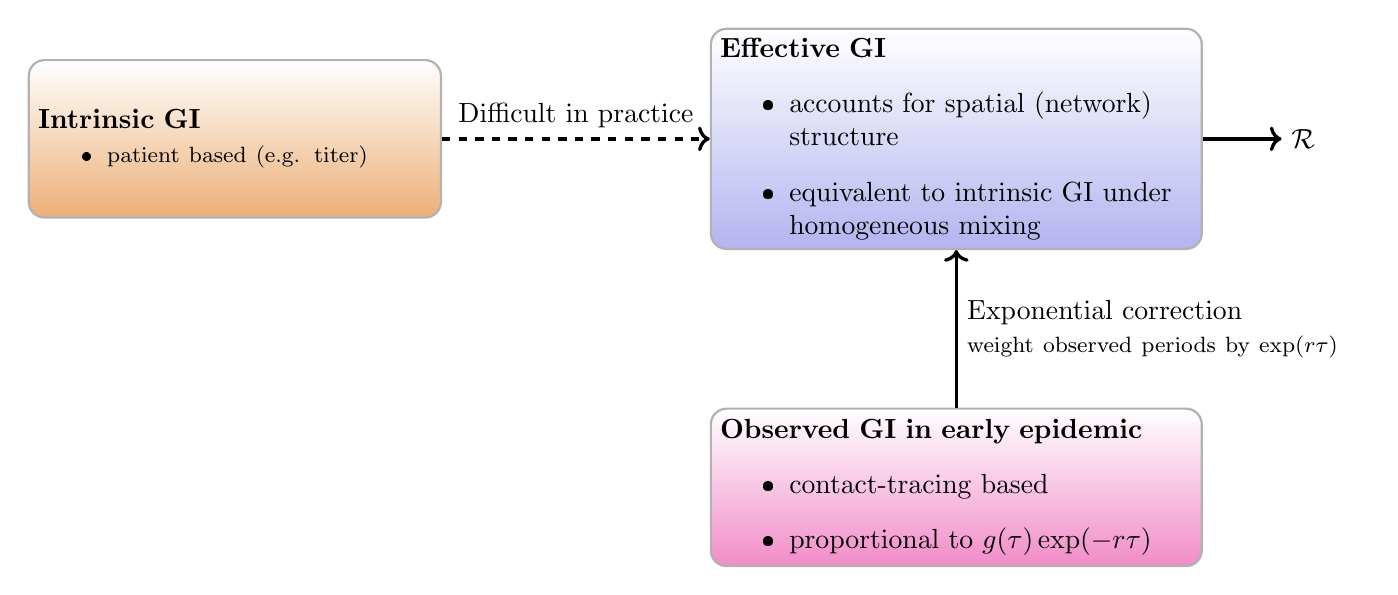
\begin{tikzpicture}
    \node(int)[bigcompartment, text width=5cm, bottom color=c1]{
    \textbf{Intrinsic GI}
    \footnotesize{
    \begin{itemize}
        \item patient based (e.g. titer)
    \end{itemize}
    }
    };
    \node(eff)[bigcompartment, right=3.4cm of int, text width=6cm, bottom color=c2]{
    \textbf{Effective GI}
    \begin{itemize}
        \item accounts for spatial (network) structure
        \item equivalent to intrinsic GI under homogeneous mixing
    \end{itemize}
    };
    \draw[->, very thick, dashed] (int) -- node [midway, above] {Difficult in practice} (eff); 
    \node(obs)[bigcompartment, below=2cm of eff, text width=6cm, bottom color=c3]{
    \textbf{Observed GI in early epidemic}
    \begin{itemize}
        \item contact-tracing based
        \item proportional to $g(\tau) \exp(-r\tau)$
    \end{itemize}
    };
    \draw[->, very thick] (obs.north) -- node [text width=5cm, midway, right] {Exponential correction\\ \footnotesize{weight observed periods by $\exp(r\tau)$}} (eff);
    \node(R)[right=of eff]{$\mathcal{R}$};
    \draw[->, very thick] (eff) -- (R);
    % \node(patient)[above left=0cm and 0.2cm of int, rotate=90]{Patient based};
\end{tikzpicture}

\end{document}
